Какому из чисел $\dfrac{2}{9}$, $-\dfrac{37}{9}$, $-\dfrac{15}{9}$, $-\dfrac{21}{9}$ соответствует точка $A$?
\begin{center}
	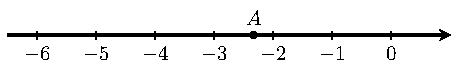
\includegraphics{graphs/graph_4/graph_4}
\end{center}

\textit{В ответе укажите номер правильного варианта.}
\begin{multicols}{4}
	\begin{enumerate}[label=\arabic*)]
		\item $\dfrac{2}{9}$
		\item $-\dfrac{15}{9}$
		\item $-\dfrac{21}{9}$
		\item $-\dfrac{37}{9}$
	\end{enumerate}
\end{multicols}